\documentclass[a4paper, 12pt]{article}

\usepackage[english]{babel}
%\usepackage[portuges]{babel}
\usepackage[utf8]{inputenc}
\usepackage{amsmath}
\usepackage{indentfirst}
\usepackage{graphicx}
\usepackage{multicol,lipsum}
%\renewcommand{\figurename}{Figura}
\usepackage{hyperref}
\usepackage{rotating}
\usepackage{lscape}

\setlength{\parskip}{1em}

\begin{document}
%\maketitle

\begin{titlepage}
	\begin{center}
	
	%\begin{figure}[!ht]
	%\centering
	%\includegraphics[width=2cm]{c:/ufba.jpg}
	%\end{figure}

		\textbf{\Large{BRP Report}}\\
		\large{Data Quality Analyst}\\ 
		%\large{Programa}\\ 
		\vspace{15pt}
        \vspace{95pt}
        %\textbf{\large{Rascunho PEP}}\\
		%\title{{\large{Título}}}
		\vspace{3,5cm}
	\end{center}
	
	\begin{flushleft}
		\begin{tabbing}
			Kallil de Araujo Bezerra \\
	\end{tabbing}
 \end{flushleft}
	\vspace{1cm}
	
	\begin{center}
		\vspace{\fill}
			\today
	\end{center}
\end{titlepage}
%%%%%%%%%%%%%%%%%%%%%%%%%%%%%%%%%%%%%%%%%%%%%%%%%%%%%%%%%%%

% % % % % % % % %FOLHA DE ROSTO % % % % % % % % % %

% % % % % % % % % % % % % % % % % % % % % % % % % %
\newpage
\tableofcontents
\thispagestyle{empty}

\newpage
\pagenumbering{arabic}
% % % % % % % % % % % % % % % % % % % % % % % % % % %
\section{Task 1 - Reading data}

The first part of the assignment is to read the data sent and do a quick analysis, to understand what this data is about. There are two files, both in \textit{.csv} format.


\begin{enumerate}
    \item What are the 10 most expensive products in the company?
    \item What sections do the \textbf{BEBIDAS} and \textbf{PADARIA} departments have?
    \item What was the total sale of products (in \$) of each Business Area in the first quarter or 2019?
\end{enumerate}

\begin{itemize}
    \item item 1
    \item item 2
    \item item 3
      \begin{itemize}
          \item sub item 1 
          \item sub item 2
          \item sub item 3
    \end{itemize}
    \item item 4
        \begin{enumerate}
            \item passo 1
            \item passo 2
            \item passo 3
        \end{enumerate}
\end{itemize}

\newpage
\subsection{Most expensive products at the company}

To analyze the most expensive products in the schema, it was necessary to order them by their prices. From most to less expensive. The query used can be seen below. The \textbf{LIMIT 11} was used because the last products cost the same (315.90), so I considered both as the $10^{th}$ position.

\begin{verbatim}
    SELECT PRODUCT_NAME, PRODUCT_VAL
    FROM looqbox_challenge.data_product
    ORDER BY PRODUCT_VAL DESC
    LIMIT 11;
\end{verbatim}

The result can be seen in the image \ref{fig_texto_jogo} or in the table \ref{tab:prod_prices}.

\begin{figure}[htb]
	\caption{\label{fig_texto_jogo} Data from task 1}
	\begin{center}
		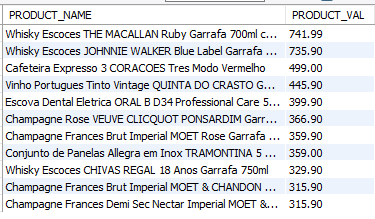
\includegraphics[scale=1.10]{task_1_sql.PNG}
	\end{center}
\end{figure}


\newpage

I tried to execute another query, using \textbf{RANK}. However, it did not work because of a server version issue. I am not sure why. The \textit{better} query is the one below, it is more elegant than the one I presented.

\begin{verbatim}
SELECT RANK() OVER(ORDER BY PRODUCT_VAL DESC) ranked_products,
       PRODUCT_NAME,
       PRODUCT_VAL
FROM looqbox_challenge.data_product
WHERE ranked_products < 10;
\end{verbatim}
\newpage
\subsection{Sections from selected departments}

In the next task it is asked to analyze which sections the departments \textbf{BEBIDAS} and \textbf{PADARIA} have. To do this, the following query was written.

\begin{verbatim}
    SELECT DISTINCT SECTION_NAME, SECTION_COD, DEP_NAME
    FROM looqbox_challenge.data_product
    WHERE (DEP_NAME LIKE 'BEBIDAS%' OR DEP_NAME LIKE 'PADARIA%')
    ORDER BY DEP_NAME;
\end{verbatim}

The result can be seen in the table \ref{tab:sections_table}.

\begin{table}[htb]
\centering
\begin{tabular}{lcc}
\hline
\# SECTION\_NAME   & \multicolumn{1}{l}{SECTION\_COD} & \multicolumn{1}{l}{DEP\_NAME} \\ \hline
BEBIDAS            & 4                                & BEBIDAS                       \\ \hline
CERVEJAS           & 29                               & BEBIDAS                       \\ \hline
VINHOS             & 30                               & BEBIDAS                       \\ \hline
REFRESCOS          & 31                               & BEBIDAS                       \\ \hline
DOCES-E-SOBREMESAS & 8                                & PADARIA                       \\ \hline
PADARIA            & 19                               & PADARIA                       \\ \hline
QUEIJOS-E-FRIOS    & 22                               & PADARIA                       \\ \hline
GESTANTE           & 27                               & PADARIA                       \\ \hline
\end{tabular}
\caption{Department and section analysis}
\label{tab:sections_table}
\end{table}

\newpage
\subsection{Total sales in 2019}
In this analysis it was assumed that Business Area could be interpreted as \textbf{BUSINESS\_NAME}.

\begin{verbatim}
    SELECT BUSINESS_NAME, SUM(SALES_VALUE)
    FROM looqbox_challenge.data_store_sales d_sales
    INNER JOIN looqbox_challenge.data_store_cad d_cad 
               ON d_cad.STORE_CODE = d_sales.STORE_CODE
    WHERE DATE BETWEEN '2019-01-01' AND '2019-04-01'
    GROUP BY BUSINESS_NAME;
\end{verbatim}

The result of this query can be seen in table \ref{tab:total_sales}. This option is ordered by the business' name. Another way to see the results is shown in the table \ref{tab:total_sales_ordered}, which is ordered by \textbf{SALES\_VALUE}, therefore the ones with highest sales value will come first.

\begin{table}[htb]
\centering
\begin{tabular}{cr}
\hline
\multicolumn{1}{l}{\# BUSINESS\_NAME} & \multicolumn{1}{l}{SUM(SALES\_VALUE)} \\ \hline
Atacado                               & 81079295.20                           \\ \hline
Farma                                 & 82462460.37                           \\ \hline
Posto                                 & 32338509.96                           \\ \hline
Proximidade                           & 80863761.30                           \\ \hline
Varejo                                & 81733342.62                           \\ \hline
\end{tabular}
\caption{Total sales by business area in the first quarter of 2019}
\label{tab:total_sales}
\end{table}

\begin{table}[htb]
\centering
\begin{tabular}{cr}
\hline
\# BUSINESS\_NAME & SUM(SALES\_VALUE) \\ \hline
Posto             & 32338509.96       \\ \hline
Proximidade       & 80863761.30       \\ \hline
Atacado           & 81079295.20       \\ \hline
Varejo            & 81733342.62       \\ \hline
Farma             & 82462460.37       \\ \hline
\end{tabular}
\caption{Total sales by business area in the first quarter of 2019 - ordered by sales value}
\label{tab:total_sales_ordered}
\end{table}

\newpage



\section{Case 1 - Dynamic Function}



\newpage
\section{Case 2 - Join queries}

Two different queries were given, and I was asked to not modify the queries. The result must be in the following format: \textbf{Loja}, \textbf{Categoria}, and \textbf{TM}. 

\begin{verbatim}
SELECT store_cad.STORE_NAME AS Loja, 
       store_cad.BUSINESS_NAME AS Categoria, 
       ROUND((store_sales.SALES_VALUE/store_sales.SALES_QTY),2) AS TM
FROM(
SELECT
      STORE_CODE,
      STORE_NAME,
      START_DATE,
      END_DATE,
      BUSINESS_NAME,
      BUSINESS_CODE
FROM looqbox_challenge.data_store_cad
) AS store_cad
JOIN (
SELECT
        STORE_CODE,
        DATE,
        SALES_VALUE,
        SALES_QTY
FROM looqbox_challenge.data_store_sales
WHERE DATE BETWEEN '2019-01-01' AND '2019-12-31'
) AS store_sales ON store_sales.STORE_CODE = store_cad.STORE_CODE
GROUP BY store_cad.STORE_NAME
ORDER BY store_cad.STORE_NAME;
\end{verbatim}


\newpage
\section{Case 3 - Data visualization}


\newpage
\end{document}



